Certainly! Below is a TikZ LaTeX code that generates the diagrams you described:

```latex
\documentclass[tikz,border=10pt]{standalone}
\usepackage{tikz}
\usetikzlibrary{shapes.geometric, arrows.meta}

\tikzset{
    block/.style={rectangle, draw=black, fill=white, text width=5em, text centered, rounded corners, minimum height=4em},
    line/.style={draw, thick, -Stealth},
    node distance=3cm,
    >=Stealth
}

\begin{document}
\begin{figure}[h]
    \centering
    \begin{minipage}{0.45\textwidth}
        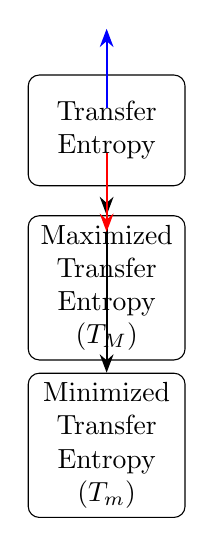
\begin{tikzpicture}[node distance=2cm]
            % Nodes
            \node (Tp) [block] {Transfer Entropy};
            \node (TM) [block, below of=Tp] {Maximized Transfer Entropy ($T_M$)};
            \node (Tm) [block, below of=TM] {Minimized Transfer Entropy ($T_m$)};
            
            % Arrows
            \draw [line] (Tp) -- (TM);
            \draw [line] (Tp) -- (Tm);
            
            % Redundant and Synergistic Influences
            \draw [red, thick, ->] (Tp.north) ++(0,-1) -- ++(0,-1);
            \draw [blue, thick, ->] (Tp.south) ++(0,1) -- ++(0,1);
        \end{tikzpicture}
        \caption*{\textbf{Left}}
    \end{minipage}
    \hspace{0.1\textwidth}
    \begin{minipage}{0.45\textwidth}
        \begin{tikzpicture}[node distance=2cm]
            % Nodes
            \node (A) [block] {Node A};
            \node (B) [block, right of=A] {Node B};
            \node (C) [block, below of=A] {Node C};
            \node (D) [block, below of=B] {Node D};
            
            % Simulated Couplings
            \draw [dashed, gray, thick, ->] (A) -- (B);
            \draw [dashed,